\documentclass[
11pt, % The default document font size, options: 10pt, 11pt, 12pt
%codirector, % Uncomment to add a codirector to the title page
]{charter} 




% El títulos de la memoria, se usa en la carátula y se puede usar el cualquier lugar del documento con el comando \ttitle
\titulo{Sistema de gestión remota de ganado} 

% Nombre del posgrado, se usa en la carátula y se puede usar el cualquier lugar del documento con el comando \degreename
%\posgrado{Carrera de Especialización en Sistemas Embebidos} 
\posgrado{Carrera de Especialización en Internet de las Cosas} 
%\posgrado{Carrera de Especialización en Intelegencia Artificial}
%\posgrado{Maestría en Sistemas Embebidos} 
%\posgrado{Maestría en Internet de las cosas}

% Tu nombre, se puede usar el cualquier lugar del documento con el comando \authorname
\autor{Ing. Ignacio Pablo Hernandorena} 

% El nombre del director y co-director, se puede usar el cualquier lugar del documento con el comando \supname y \cosupname y \pertesupname y \pertecosupname
\director {Mg. Ing. Carlos Canal (pendiente aprobación)}
\pertenenciaDirector{UNSAM} 
% FIXME:NO IMPLEMENTADO EL CODIRECTOR ni su pertenencia
%\codirector{John Doe} % para que aparezca en la portada se debe descomentar la opción codirector en el documentclass
%\pertenenciaCoDirector{FIUBA}

% Nombre del cliente, quien va a aprobar los resultados del proyecto, se puede usar con el comando \clientename y \empclientename
\cliente{-}
\empresaCliente{Empresas o personas en el rubro ganadero}

% Nombre y pertenencia de los jurados, se pueden usar el cualquier lugar del documento con el comando \jurunoname, \jurdosname y \jurtresname y \perteunoname, \pertedosname y \pertetresname.
\juradoUno{Nombre y Apellido (1)}
\pertenenciaJurUno{pertenencia (1)} 
\juradoDos{Nombre y Apellido (2)}
\pertenenciaJurDos{pertenencia (2)}
\juradoTres{Nombre y Apellido (3)}
\pertenenciaJurTres{pertenencia (3)}
 
\fechaINICIO{25 de abril de 2023}		%Fecha de inicio de la cursada de GdP \fechaInicioName
\fechaFINALPlan{13 de junio de 2023} 	%Fecha de final de cursada de GdP
\fechaFINALTrabajo{02 de febrero de 2024}	%Fecha de defensa pública del trabajo final


\begin{document}

\maketitle
\thispagestyle{empty}
\pagebreak


\thispagestyle{empty}
{\setlength{\parskip}{0pt}
\tableofcontents{}
}
\pagebreak


\section*{Registros de cambios}
\label{sec:registro}


\begin{table}[ht]
\label{tab:registro}
\centering
\begin{tabularx}{\linewidth}{@{}|c|X|c|@{}}
\hline
\rowcolor[HTML]{C0C0C0} 
Revisión & \multicolumn{1}{c|}{\cellcolor[HTML]{C0C0C0}Detalles de los cambios realizados} & Fecha      \\ \hline
0      & Creación del documento                                 &\fechaInicioName \\ \hline
1      & Se completa hasta el punto 5 inclusive                 & 09 de mayo de 2023 \\ \hline
2      & Se completa hasta el punto 9 inclusive				   & 16 de mayo de 2023 \\ \hline
3      & Se completa hasta el punto 12 inclusive                & 23 de mayo de 2023  \\ \hline
4      & Se completa el plan	                                   & 30 de mayo de 2023 \\ \hline
\end{tabularx}
\end{table}

\pagebreak



\section*{Acta de constitución del proyecto}
\label{sec:acta}

\begin{flushright}
Buenos Aires, \fechaInicioName
\end{flushright}

\vspace{2cm}

Por medio de la presente se acuerda con el \authorname\hspace{1px} que su Trabajo Final de la \degreename\hspace{1px} se titulará ``\ttitle'', consistirá esencialmente en la implementación de un prototipo de un sistema de gestión remota de ganado, y tendrá un presupuesto preliminar estimado de 610 horas de trabajo y USD 9015,85, con fecha de inicio \fechaInicioName\hspace{1px} y fecha de presentación pública \fechaFinalName.

Se adjunta a esta acta la planificación inicial.

\vfill

% Esta parte se construye sola con la información que hayan cargado en el preámbulo del documento y no debe modificarla
\begin{table}[ht]
\centering
\begin{tabular}{ccc}
\begin{tabular}[c]{@{}c@{}}Dr. Ing. Ariel Lutenberg \\ Director posgrado FIUBA\end{tabular} & \hspace{2cm} & \begin{tabular}[c]{@{}c@{}}\clientename \\ \empclientename \end{tabular} \vspace{2.5cm} \\ 
\multicolumn{3}{c}{\begin{tabular}[c]{@{}c@{}} \supname \\ Director del Trabajo Final\end{tabular}} \vspace{2.5cm} \\
%\begin{tabular}[c]{@{}c@{}}\jurunoname \\ Jurado del Trabajo Final\end{tabular}     &  & \begin{tabular}[c]{@{}c@{}}\jurdosname\\ Jurado del Trabajo Final\end{tabular}  \vspace{2.5cm}  \\
%\multicolumn{3}{c}{\begin{tabular}[c]{@{}c@{}} \jurtresname\\ Jurado del Trabajo Final\end{tabular}} \vspace{.5cm}                                                                     
\end{tabular}
\end{table}




\section{1. Descripción técnica-conceptual del proyecto a realizar}
\label{sec:descripcion}

La tecnología IoT (del inglés \emph{Internet of Things}) ha revolucionado muchas industrias, incluida la agrícola y ganadera. El desarrollo de sistemas de gestión de ganado utilizando IoT ayuda al personal rural a monitorear y controlar sus tierras y animales, proporcionando así condiciones óptimas para el progreso de esta actividad.

Hoy existe una demanda de este tipo de tecnología en Argentina, donde la ganadería es una parte importante de la economía. Algunos de los desafíos comunes que enfrentan los propietarios y cuidadores de ganado es controlar que los animales no deambulen y se pierdan, o que causen daños a los cultivos y a otras propiedades.

Mediante el uso de la tecnología IoT se puede desarrollar un dispositivo que ayude a mantener al ganado en su lugar. Si a esto se le suma la posibilidad de mantener un registro completo de cada animal se obtiene una solución integral para el propietario.

Para abordar esta problemática se propone la implementación de un prototipo que utilizará un sistema IoT para la gestión remota de ganado. Cabe mencionar que este proyecto se trata de una iniciativa personal, con el objetivo de contribuir al avance en el ámbito de la tecnología y la ganadería.

El sistema consta de etiquetas electrónicas (en adelante denominados \emph{TAGs}) que serán fijadas en las orejas de los animales. Para ello, se utilizarán dispositivos de bajo consumo de energía que emplean la tecnología de red de largo alcance conocida como LoRaWAN. Además, se desarrollará una plataforma que permitirá gestionar, controlar, almacenar y visualizar los datos generados por estos dispositivos.

Como se puede observar en la figura \ref{fig:diagBloques}, para implementar este sistema se requieren diversos componentes, como los \emph{TAGs}. Los mismos estarán compuestos de un panel solar, un sistema de alimentación, el GPS (del inglés \emph{Global Positioning System}) y el dispositivo con LoRaWAN que obtendrá los datos y los enviará a un gateway. 

El gateway actuará recopilando y procesando la información de los \emph{TAGs} y enviándola a una base de datos remota. Este dispositivo requerirá una conexión a internet para la vinculación con la plataforma en la nube llamada \emph{The Things Stack}.

\emph{The Things Stack} es un servidor de red LoRaWAN altamente escalable y de código abierto que permite que las aplicaciones y los servicios de IoT conecten y administren dispositivos, datos y aplicaciones de manera segura. 

\begin{figure}[htpb]
\centering 
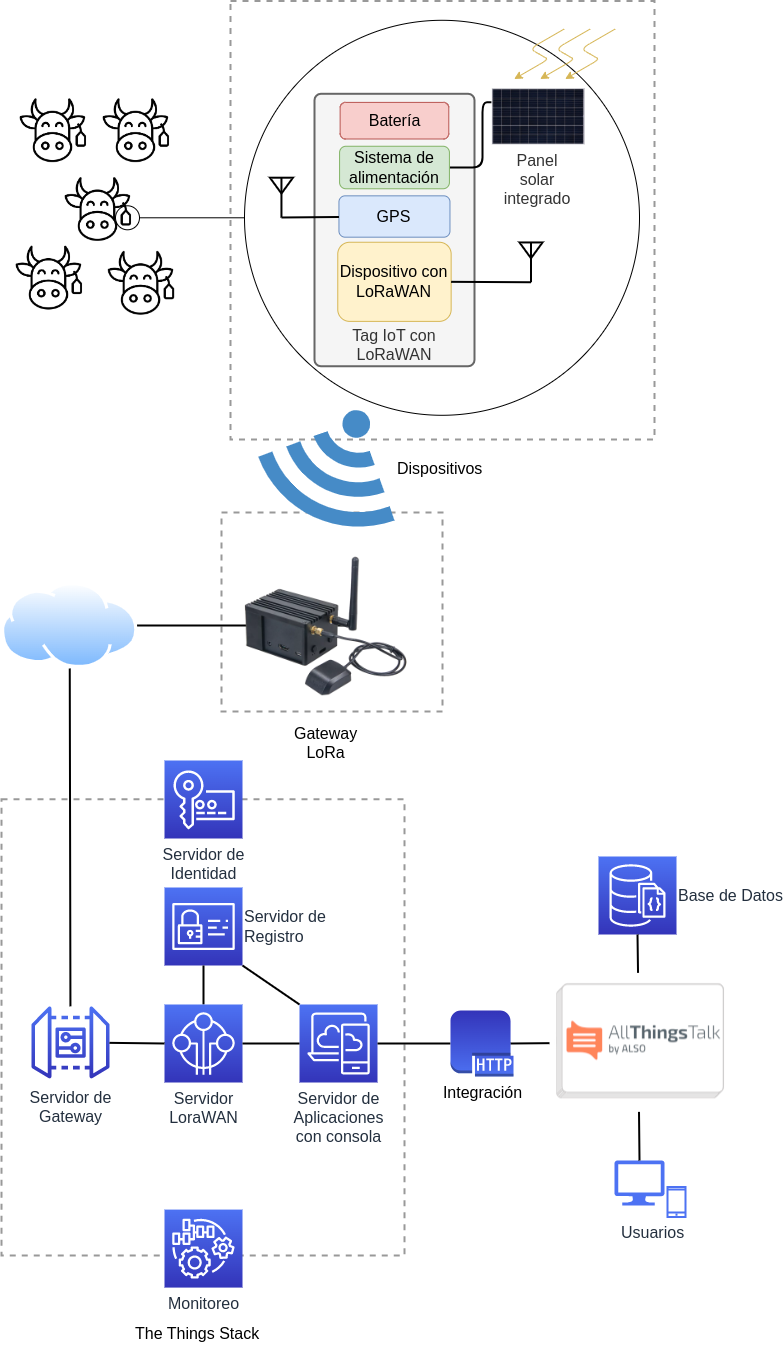
\includegraphics[width=.7\textwidth]{./Figuras/diagBloques.png}
\caption{Diagrama en bloques del sistema}
\label{fig:diagBloques}
\end{figure}

\emph{The Things Stack} ofrece una amplia gama de servicios para admitir aplicaciones IoT, dentro de los que se incluyen: 
\begin{itemize}
	\item Servidor de gateway: proporciona herramientas para administrar dispositivos y sus datos asociados, incluida la activación, el registro y la autorización de dispositivos.
	\item Servidor de identidad: ofrece características de seguridad avanzadas, incluido el cifrado de extremo a extremo y protocolos de comunicación seguros, para garantizar la privacidad y seguridad de los datos de IoT.
	\item Servidor LoRaWAN: es el encargado de recibir y procesar datos de dispositivos IoT y de administrar la activación, la seguridad y el cifrado de datos del dispositivo. Además permite la recopilación, el almacenamiento y el análisis de datos generados por los dispositivos IoT.
	\item Servidor de registro: es responsable de autorizar de forma segura nuevos dispositivos para conectarse a la red y de administrar el proceso de autenticación de dispositivos.
	\item Servidor de aplicaciones: debe procesar y enrutar los datos de los dispositivos a las aplicaciones o servicios apropiados.
	\item Monitoreo:
		\begin{itemize}
		\item Tablero: consiste en un tablero personalizable que muestra información en tiempo real sobre el rendimiento de la red, la actividad del dispositivo y el uso de datos.
		\item Eventos: se pueden visualizar alertas y notificaciones para eventos clave, como activación de dispositivos, transmisión de datos y problemas de rendimiento de la red.
		\end{itemize}
	\item Integración: ofrece una variedad de opciones de integración para conectarse con otros sistemas, como otras plataformas en la nube, bases de datos y herramientas de análisis. Para este proyecto se realizará una integración mediante HTTP (del inglés \emph{Hypertext Transfer Protocol}) a \emph{AllThingsTalk}.
\end{itemize}

\emph{AllThingsTalk} es una plataforma de IoT basada en la nube que proporciona una variedad de herramientas y servicios para crear, implementar y administrar aplicaciones y dispositivos de IoT. Esta plataforma ofrece una interfaz fácil de usar y un conjunto de componentes básicos personalizables, lo que facilita la creación y el escalado de soluciones de IoT para una variedad de industrias y casos de uso. 

Los usuarios utilizarán la plataforma para delimitar las áreas permitidas para la circulación de los animales, establecer las alarmas y monitorear el ganado en tiempo real. Además, se establecerá la conexión de la aplicación generada en \emph{AllThingsTalk} a una base de datos donde se guardará el registro médico de cada animal. 


\section{2. Identificación y análisis de los interesados}
\label{sec:interesados}

\begin{table}[ht]
%\caption{Identificación de los interesados}
%\label{tab:interesados}
\begin{tabularx}{\linewidth}{@{}|l|X|X|l|@{}}
\hline
\rowcolor[HTML]{C0C0C0} 
Rol           & Nombre y Apellido & Organización 	& Puesto 	\\ \hline
Cliente       & \clientename      &\empclientename	&   -     	\\ \hline
Responsable   & \authorname       & FIUBA        	& Alumno 	\\ \hline
Orientador    & \supname	      & \pertesupname 	& Director trabajo final \\ \hline
Usuario final & Personal rural         &  -           	&   -     	\\ \hline
\end{tabularx}
\end{table}

 
Características de los interesados:
\begin{itemize}
	\item Cliente: es el propietario del ganado, ya sea una persona o una empresa que busca mejorar la gestión de sus animales mediante el uso de tecnología IoT. Este grupo de interesados espera obtener beneficios como la reducción de costos, la mejora en la calidad de vida de los animales y la disminución de pérdidas o daños causados por el ganado.
	\item Orientador: es responsable de garantizar que el proyecto cumpla con los estándares de calidad y que se sigan las mejores prácticas en el desarrollo de software y hardware. La disponibilidad horaria esta acotada de lunes a viernes de 9 a 18 hs. 
	\item Usuarios: es el personal rural encargado de cuidar y monitorear el ganado utilizando el sistema de gestión de ganado IoT.
\end{itemize}


\section{3. Propósito del proyecto}
\label{sec:proposito}

El propósito de este proyecto es desarrollar un sistema de monitoreo remoto de ganado que permita a las empresas, o personas relacionadas a este sector, tener acceso a información en tiempo real sobre la ubicación y el estado de su ganado, lo que les permitirá, en base a información detallada, mejorar la toma de decisiones y la eficiencia en la gestión. Este sistema deberá ser fácil de usar y escalable para adaptarse a cualquier tipo de establecimiento, ya sea pequeño o grande.

\section{4. Alcance del proyecto}
\label{sec:alcance}

El alcance del proyecto incluye el desarrollo de un prototipo de sistema de gestión de ganado utilizando tecnología IoT. El sistema estará compuesto de \emph{TAGs} que se fijarán en las orejas de los animales utilizando dispositivos de bajo consumo de energía con tecnología de red de largo alcance conocida como LoRaWAN. Además, se dispondrá de una plataforma en la nube llamada \emph{The Things Stack} para la gestión, el control, almacenamiento y visualización de los datos que generan estos dispositivos. Se integrará la plataforma mediante HTTP a \emph{AllThingsTalk}, que será utilizada por los usuarios para delimitar las áreas permitidas para la circulación de los animales, establecer alarmas y monitorear el ganado en tiempo real. También se establecerá la conexión de la aplicación generada en \emph{AllThingsTalk} a una base de datos donde se guardará el registro médico de cada animal.

No se incluyen en este proyecto aspectos relacionados con el desarrollo de hardware o software para dispositivos móviles. Tampoco se incluye la instalación de la infraestructura necesaria para la conexión a internet o para el uso del sistema de gestión de ganado. Asimismo, este proyecto no contempla la producción a gran escala de los \emph{TAGs} o la distribución de los mismos. 

Este proyecto se centrará únicamente en el desarrollo de un prototipo que pueda ser utilizado como una prueba de concepto para demostrar la viabilidad del sistema de gestión de ganado mediante IoT.


\section{5. Supuestos del proyecto}
\label{sec:supuestos}

Para el desarrollo del presente proyecto se supone que:

\begin{itemize}
	\item Se contará con el tiempo necesario para la realización de las tareas específicas del proyecto.
	\item Los recursos financieros necesarios para la ejecución del proyecto estarán disponibles en tiempo y forma.
	\item La tecnología y las herramientas necesarias para el desarrollo del proyecto estarán disponibles y en condiciones óptimas de funcionamiento.
	\item No habrá cambios significativos en las condiciones macroeconómicas que afecten de manera importante la ejecución del proyecto.
	\item El entorno regulatorio y normativo en el que se desarrollará el proyecto permanecerá estable y sin cambios importantes que afecten la ejecución del proyecto.
	\item Los proveedores y terceros involucrados en el proyecto cumplirán con sus compromisos en tiempo y forma.
	\item Los animales se encuentran en un radio igual o menor en el que se puede utilizar la tecnología de LoRaWAN. 
	\item Los imprevistos y cambios inesperados que puedan surgir durante el desarrollo del proyecto se abordarán de manera eficiente y efectiva para minimizar su impacto en el éxito del proyecto.
	\item Se mantendrá una comunicación clara y efectiva con los interesados involucrados en el proyecto para garantizar una adecuada coordinación y colaboración.
\end{itemize}


\section{6. Requerimientos}
\label{sec:requerimientos}

\begin{enumerate}
	\item Requerimientos funcionales
		\begin{enumerate}
			\item El sistema deberá permitir la instalación y configuración de \emph{TAGs} en las orejas de los animales.
			\item El sistema deberá utilizar dispositivos de bajo consumo de energía con tecnología LoRaWAN para la transmisión de datos.
			\item El sistema deberá recopilar y procesar la información de los \emph{TAGs} y enviarla al gateway.
			\item El sistema deberá proporcionar una plataforma para la gestión, control, almacenamiento y visualización de los datos generados por los dispositivos.
			\item El sistema deberá permitir delimitar áreas permitidas para la circulación de los animales.
			\item El sistema deberá ofrecer la posibilidad de establecer alarmas para eventos relevantes, como la salida de un animal del área permitida.
			\item El sistema deberá permitir el monitoreo en tiempo real del ganado a través de un tablero personalizable.
		\end{enumerate}
	\item Requerimientos de seguridad
		\begin{enumerate}
			\item El sistema deberá garantizar la privacidad y seguridad de los datos de IoT mediante características de seguridad avanzadas, como el cifrado de extremo a extremo y protocolos de comunicación seguros.
			\item El sistema deberá contar con un proceso de autenticación seguro para nuevos dispositivos que se conecten a la red.
		\end{enumerate}
		
	\item Requerimientos de integración
		\begin{enumerate}
			\item El sistema deberá integrarse con la plataforma en la nube \emph{The Things Stack} a través de una conexión a internet.
			\item El sistema deberá permitir la integración con otras plataformas en la nube, bases de datos y herramientas de análisis mediante HTTP, utilizando la plataforma \emph{AllThingsTalk}.
		\end{enumerate}
		
	\item Requerimientos de documentación
		\begin{enumerate}
			\item Se deberá generar documentación detallada sobre la instalación, configuración y uso del sistema.
			\item Se deberá proporcionar documentación sobre las normas y regulaciones vigentes relacionadas con el monitoreo remoto de ganado definidas por el INTA (Instituto Nacional de Tecnología Agropecuaria) .
		\end{enumerate}
	
	\item Requerimientos de la interfaz
		\begin{enumerate}			
			\item La interfaz de usuario deberá ser intuitiva y fácil de usar, las mismas se medirán de acuerdo al tiempo promedio de aprendizaje (\textless 1 hora), la tasa de errores de usuario (\textless  5 \% ) y la retroalimentación.
			\item Deberá existir un panel de control centralizado que muestre información en tiempo real sobre el estado del ganado, incluyendo ubicación, actividad y alertas.
			\item  Se deberán proporcionar herramientas de configuración y personalización de las áreas permitidas para la circulación del ganado, así como la definición de alarmas y notificaciones.
			\item La interfaz deberá permitir el acceso a un registro médico completo de cada animal, incluyendo historial de enfermedades, vacunas y tratamientos.
			\item La interfaz deberá ser compatible con los siguientes navegadores web: Chrome, Firefox, Edge y Safari.
			\item Se deberá garantizar la seguridad de la interfaz, protegiendo los datos y proporcionando mecanismos de autenticación y autorización para los usuarios.
		\end{enumerate}
		
	\item Requerimientos de \emph{testing}
		\begin{enumerate}
			\item El sistema deberá ser sometido a pruebas exhaustivas para verificar su funcionalidad y rendimiento.
			\item Se deberán realizar pruebas de integración para garantizar la correcta comunicación entre los componentes del sistema.
			\item Se deberán realizar pruebas de seguridad para identificar posibles vulnerabilidades y asegurar la protección de los datos.
			\item Se deberán documentar los resultados de las pruebas y realizar las correcciones necesarias antes de la implementación final del sistema.
		\end{enumerate}
		
\end{enumerate}


\section{7. Historias de usuarios (\textit{Product backlog})}
\label{sec:backlog}

Para determinar los \emph{story points}, se empleó una escala de Fibonacci en la cual se asignaron valores a las historias de usuario según su complejidad, dificultad e incertidumbre. En esta escala, cada número es la suma de los dos números anteriores en la secuencia de Fibonacci.

\begin{quote}
Como ganadero, quiero poder monitorear la ubicación de cada animal en tiempo real para asegurarme de que no se alejen de las áreas permitidas. \emph{Story points}: 8 (Complejidad: 5 - Dificultad: 3 - Incertidumbre: 0)
\end{quote} 

\begin{quote}
Como cuidador del ganado, quiero recibir notificaciones automáticas cuando un animal se aleje de su área permitida para poder tomar medidas inmediatas. \emph{Story points}: 13 (Complejidad: 5 - Dificultad: 5 - Incertidumbre: 3)
\end{quote} 

\begin{quote}
Como propietario de la finca, quiero poder establecer alarmas personalizadas para cada animal, como alertas de movimiento excesivo o ausencia prolongada, para garantizar su bienestar y seguridad. \emph{Story points}: 8 (Complejidad: 5 - Dificultad: 3 - Incertidumbre: 0)
\end{quote} 

\begin{quote}
Como veterinario, quiero acceder a un registro médico completo de cada animal en la plataforma para poder realizar un seguimiento adecuado de su historial de enfermedades, vacunas y tratamientos. \emph{Story points}: 5 (Complejidad: 1 - Dificultad: 3 - Incertidumbre: 1)
\end{quote} 

\begin{quote}
Como propietario del ganado, quiero tener acceso a un informe detallado del historial de ubicaciones de cada animal para poder rastrear su movimiento y analizar su comportamiento. \emph{Story points}: 8 (Complejidad: 3 - Dificultad: 3 - Incertidumbre: 2)
\end{quote} 

\begin{quote}
Como cuidador del ganado, quiero poder consultar el estado de la batería de los \emph{TAGs} en la plataforma de monitoreo para asegurarme de que están funcionando correctamente. \emph{Story points}: 5 (Complejidad: 1 - Dificultad: 3 - Incertidumbre: 1)
\end{quote}

\begin{quote}
Como usuario del sistema, quiero tener la capacidad de realizar actualizaciones remotas del firmware en los \emph{TAGs} para mejorar su funcionalidad y seguridad. \emph{Story points}: 8 (Complejidad: 3 - Dificultad: 3 - Incertidumbre: 2)
\end{quote} 


\section{8. Entregables principales del proyecto}
\label{sec:entregables}

Los entregables del proyecto son:

\begin{itemize}
	\item Informe de avance: documento que contiene una actualización sobre el progreso del presente proyecto.
	\item Manual de usuario: documento que proporciona instrucciones detalladas sobre cómo utilizar el sistema de gestión de ganado, incluyendo las funcionalidades, configuraciones y solución de problemas.
	\item Diagrama de la solución: representación gráfica de los componentes electrónicos y su interconexión en el dispositivo de gestión de ganado, incluyendo el panel solar, sistema de alimentación, GPS y dispositivo LoRaWAN.
	\item Código fuente del \emph{firmware}: conjunto de programas y \emph{scripts} necesarios para el funcionamiento del dispositivo de gestión de ganado, incluyendo la comunicación con los \emph{TAGs}, la transferencia de datos y la interacción con el gateway.
	\item Diagrama de instalación: esquema que muestra cómo se instala y configura el sistema de gestión de ganado en la finca o establecimiento ganadero, incluyendo la ubicación de los dispositivos, antenas y posibles requisitos de red.
	\item Informe final: documento que resume todo el desarrollo del proyecto, incluyendo los objetivos, metodología, resultados, conclusiones y recomendaciones. También podrá incluir detalles sobre los desafíos enfrentados, lecciones aprendidas y posibles mejoras futuras.
	\item Prototipo funcional: entrega de un prototipo del dispositivo de gestión de ganado que cumple con los requisitos y funcionalidades especificadas en el proyecto.
	\item Resultados de pruebas: informe que documenta los resultados de las pruebas realizadas al sistema de gestión de ganado, incluyendo pruebas de funcionalidad, rendimiento, estabilidad y seguridad.
\end{itemize}

\section{9. Desglose del trabajo en tareas}
\label{sec:wbs}

A continuación se presenta el WBS (\emph{del inglés Work Breakdown Structure}):

\begin{enumerate}
\item Investigación (40 horas)
	\begin{enumerate}	
	\item  Investigación de tecnologías y soluciones existentes (16 horas)
	\item  Investigación de requisitos y especificaciones adicionales (16 horas)
	\item  Análisis de viabilidad y evaluación de alternativas (8 horas)
	\end{enumerate}
\item Inicio del proyecto (40 horas)
	\begin{enumerate}
	\item Definición de objetivos y alcance del proyecto (8 horas)
	\item Identificación de interesados y requisitos (8 horas)
	\item Elaboración del plan de proyecto y asignación de recursos (20 horas)
	\item Reunión con el director del proyecto (4 horas)
	\end{enumerate}
\item Análisis y diseño (108 horas)
	\begin{enumerate}
	\item Revisión de requerimientos y especificaciones (16 horas)
	\item Diseño de la arquitectura del sistema (20 horas)
	\item Diseño de la interfaz de usuario (24 horas)
	\item Evaluación y selección de componentes electrónicos (20 horas)
	\item Diseño de la estructura de datos y bases de datos (24 horas)
	\item Reunión con el director del proyecto (4 horas)
	\end{enumerate}
\item Desarrollo del \emph{firmware} y \emph{software} (220 horas)
	\begin{enumerate}
	\item Adquisición de los componentes y ensamblaje del dispositivo (24 horas)
	\item Programación del firmware del dispositivo IoT (50 horas)
	\item Desarrollo de la plataforma de gestión y control (50 horas)
	\item Implementación de la comunicación LoRaWAN (32 horas)
	\item Integración con \emph{The Things Stack} y \emph{AllThingsTalk} (24 horas)
	\item Desarrollo de la interfaz de usuario (20 horas)
	\item Pruebas unitarias y depuración (16 horas)
	\item Reunión con el director del proyecto (4 horas)
	\end{enumerate}
\item Implementación y pruebas (100 horas)
	\begin{enumerate}
	\item Configuración y despliegue del gateway LoRaWAN (24 horas)
	\item Instalación y configuración del sistema de prueba (24 horas)
	\item Pruebas de integración y funcionamiento del sistema (24 horas)
	\item Pruebas de conectividad y transmisión de datos (16 horas)
	\item Pruebas de rendimiento y estabilidad del sistema (8 horas)
	\item Reunión con el director del proyecto (4 horas)
	\end{enumerate}
\item Documentación y entrega (102 horas)
	\begin{enumerate}
	\item Elaboración del informe de avance (14 horas)
	\item Documentación técnica del proyecto y sistema (24 horas)
	\item Elaboración del manual de usuario (20 horas)
	\item Preparación de la presentación final (20 horas)
	\item Revisión y validación de los entregables (12 horas)
	\item Reunión con el director del proyecto (4 horas)
	\item Demostración del sistema a los interesados (4 horas)
	\item Cierre del proyecto y evaluación de lecciones aprendidas (4 horas)
	\end{enumerate}
\end{enumerate}

Cantidad total de horas: 610 horas


\vspace*{\fill}
\pagebreak
\section{10. Diagrama de Activity On Node}
\label{sec:AoN}

\begin{figure}[htpb]
\centering 
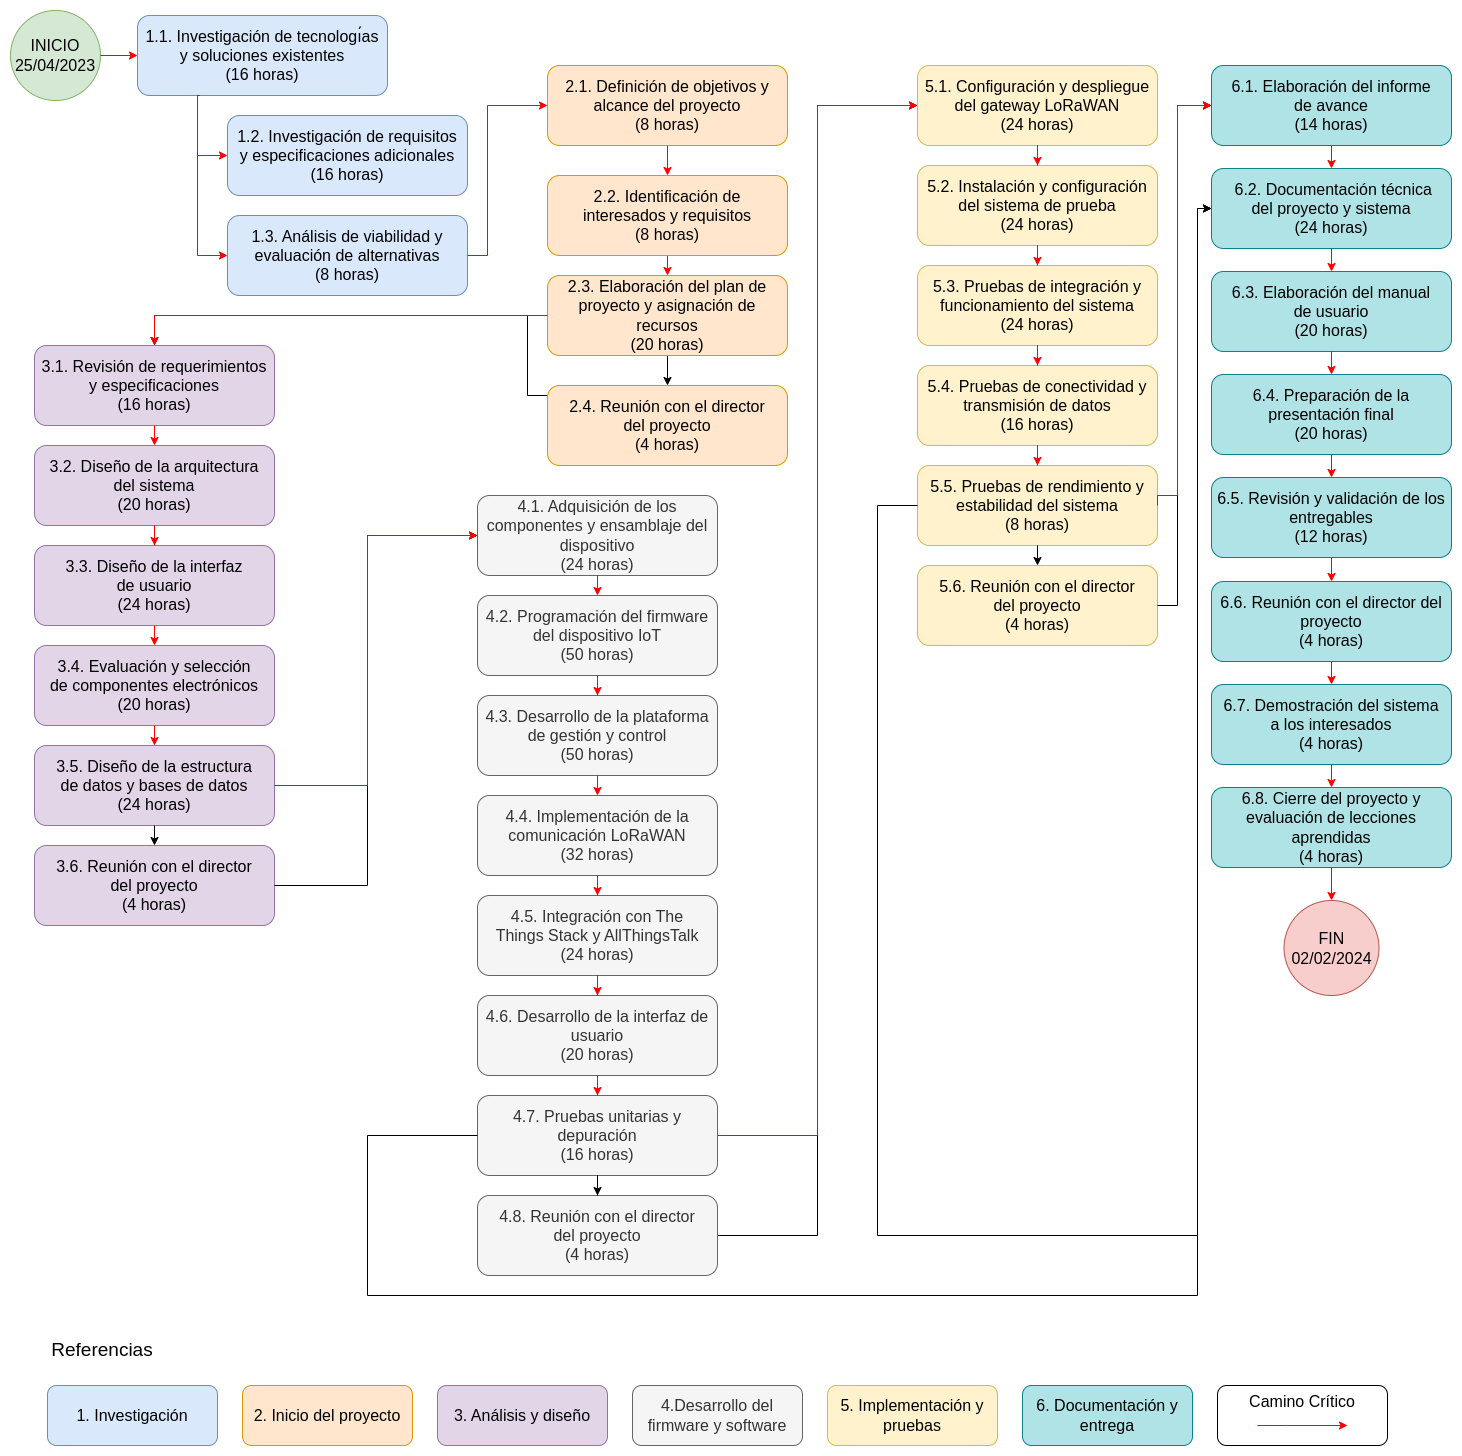
\includegraphics[width=1.1\textwidth]{./Figuras/AoN.png}
\caption{Diagrama de \textit{Activity on Node}.}
\label{fig:AoN}
\end{figure}



\section{11. Diagrama de Gantt}
\label{sec:diagGantt}

A partir del WBS y del AoN definido en las secciones anteriores se establece el diagrama de Gantt como se puede observar a continuación en la figura \ref{fig:diagGantt}.

\begin{landscape}
\begin{figure}[htpb]
\centering 
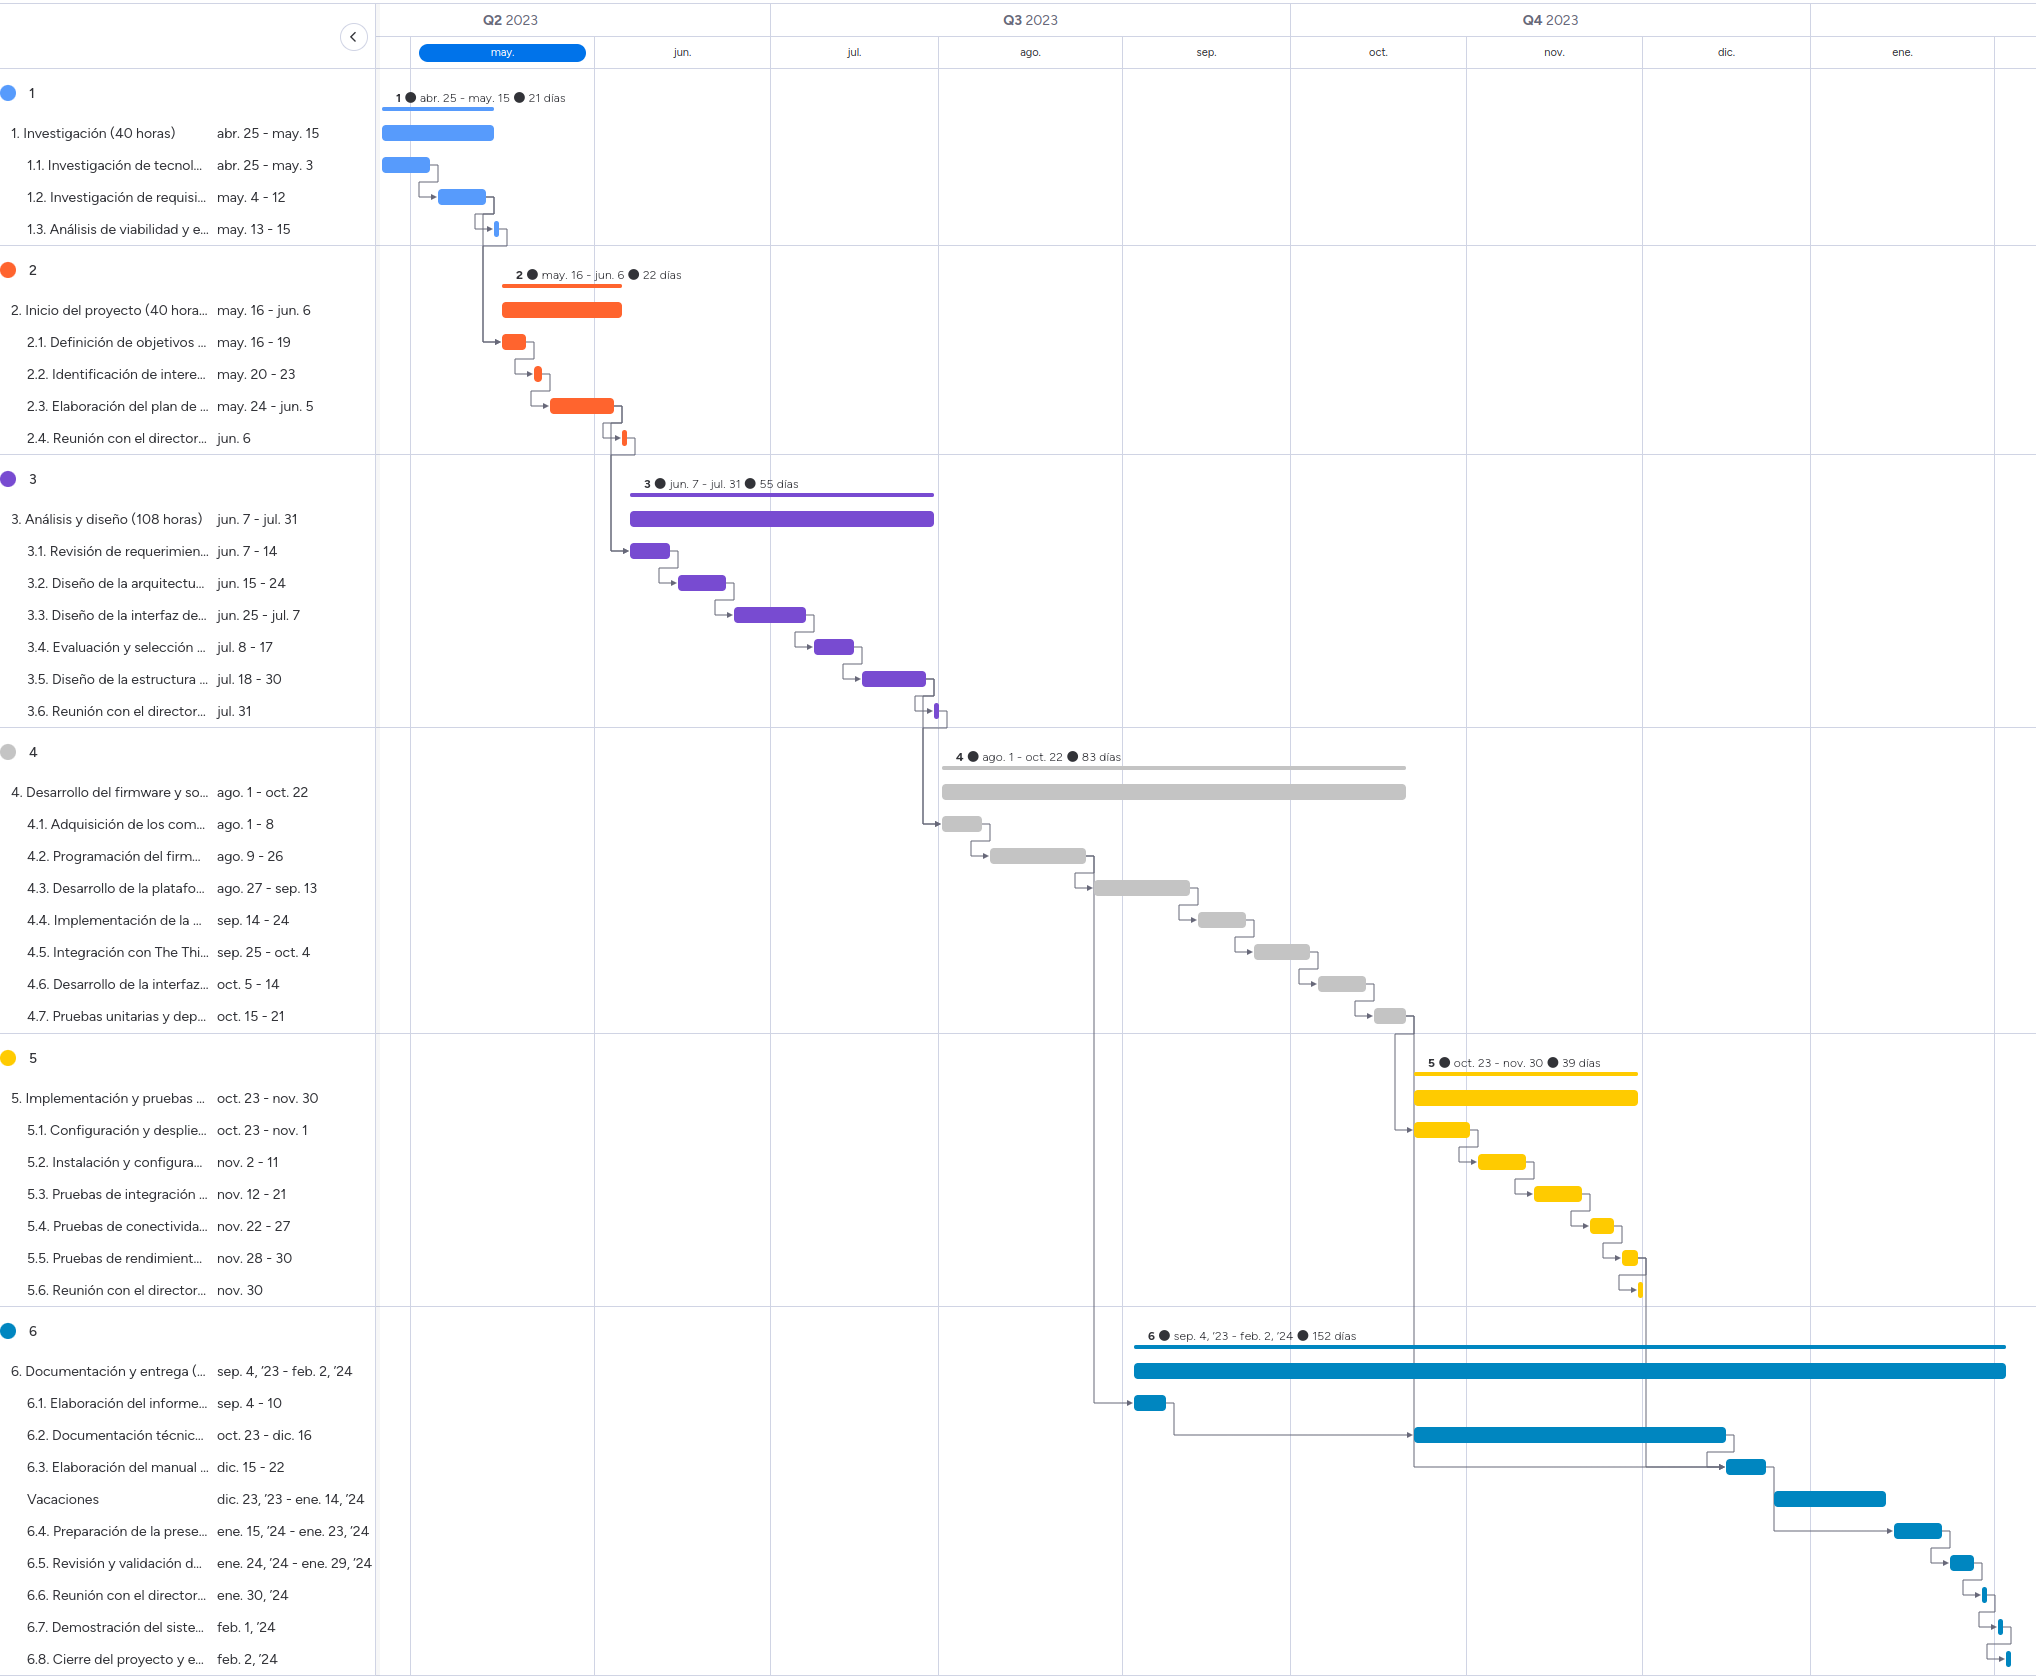
\includegraphics[height=1\textheight]{./Figuras/Gantt-2.png}
\caption{Diagrama de Gantt}
\label{fig:diagGantt}
\end{figure}

\end{landscape}




\section{12. Presupuesto detallado del proyecto}
\label{sec:presupuesto}

Los costos del presente proyecto se estimaron en dolares estadounidenses. Al momento de elaborar este documento el valor de cotización es USD 1 = \$ 487,00. 

\begin{table}[htpb]
\centering
\begin{tabularx}{\linewidth}{@{}|X|c|r|r|@{}}
\hline
\rowcolor[HTML]{C0C0C0} 
\multicolumn{4}{|c|}{\cellcolor[HTML]{C0C0C0}COSTOS DIRECTOS} \\ \hline
\rowcolor[HTML]{C0C0C0} 
Descripción &
  \multicolumn{1}{c|}{\cellcolor[HTML]{C0C0C0}Cantidad} &
  \multicolumn{1}{c|}{\cellcolor[HTML]{C0C0C0}Valor unitario} &
  \multicolumn{1}{c|}{\cellcolor[HTML]{C0C0C0}Valor total} \\ \hline
  
  \multicolumn{1}{|l|}{Modulo WiFi LoRa 32 (V3)} &
  \multicolumn{1}{c|}{1} &
  \multicolumn{1}{c|}{USD 25,40} &
  \multicolumn{1}{c|}{USD 25,40} \\ \hline
  
  \multicolumn{1}{|l|}{Gateway RAK7243 WisGate Developer D3} &
  \multicolumn{1}{c|}{1} &
  \multicolumn{1}{c|}{USD 252,73} &
  \multicolumn{1}{c|}{USD 252,73} \\ \hline
  
  \multicolumn{1}{|l|}{Fuente de alimentación 5V} &
  \multicolumn{1}{c|}{1} &
  \multicolumn{1}{c|}{USD 6,35} &
  \multicolumn{1}{c|}{USD 6,35} \\ \hline
  
  \multicolumn{1}{|l|}{Cable micro USB} &
  \multicolumn{1}{c|}{1} &
  \multicolumn{1}{c|}{USD 1,85} &
  \multicolumn{1}{c|}{USD 1,85} \\ \hline
  
  \multicolumn{1}{|l|}{Protoboard} &
  \multicolumn{1}{c|}{1} &
  \multicolumn{1}{c|}{USD 5,12} &
  \multicolumn{1}{c|}{USD 5,12} \\ \hline
  
  \multicolumn{1}{|l|}{Batería TR 14500 3.7v 1500mAh} &
  \multicolumn{1}{c|}{1} &
  \multicolumn{1}{c|}{USD 5,64} &
  \multicolumn{1}{c|}{USD 5,64} \\ \hline  
   
  \multicolumn{1}{|l|}{Panel solar 5V 200mA} &
  \multicolumn{1}{c|}{1} &
  \multicolumn{1}{c|}{USD 7,21} &
  \multicolumn{1}{c|}{USD 7,21} \\ \hline  
  
  \multicolumn{1}{|l|}{Modulo GPS GY-NEO6MV2} &
  \multicolumn{1}{c|}{1} &
  \multicolumn{1}{c|}{USD 9,12} &
  \multicolumn{1}{c|}{USD 9,12} \\ \hline    
  
  \multicolumn{1}{|l|}{Kit 40 cables Dupont} &
  \multicolumn{1}{c|}{1} &
  \multicolumn{1}{c|}{USD 5,47} &
  \multicolumn{1}{c|}{USD 5,47} \\ \hline  
  
  \multicolumn{1}{|l|}{Horas de ingeniería} &
  \multicolumn{1}{c|}{610} &
  \multicolumn{1}{c|}{USD 10} &
  \multicolumn{1}{c|}{USD 6100} \\ \hline

  \multicolumn{3}{|c|}{SUBTOTAL} &
  \multicolumn{1}{c|}{USD 6439,89} \\ \hline
  \rowcolor[HTML]{C0C0C0} 

\multicolumn{4}{|c|}{\cellcolor[HTML]{C0C0C0}COSTOS INDIRECTOS} \\ \hline
\rowcolor[HTML]{C0C0C0} 
Descripción &
  \multicolumn{1}{c|}{\cellcolor[HTML]{C0C0C0}Cantidad} &
  \multicolumn{1}{c|}{\cellcolor[HTML]{C0C0C0}Valor unitario} &
  \multicolumn{1}{c|}{\cellcolor[HTML]{C0C0C0}Valor total} \\ \hline
  
  \multicolumn{1}{|l|}{40 \% de los costos directos} &
  \multicolumn{1}{c|}{1} &
  \multicolumn{1}{c|}{USD 2575,96} &
  \multicolumn{1}{c|}{USD 2575,96} \\ \hline

\multicolumn{3}{|c|}{SUBTOTAL} &
  \multicolumn{1}{c|}{USD 2575,96} \\ \hline
\rowcolor[HTML]{C0C0C0}
\multicolumn{3}{|c|}{TOTAL} &
  \multicolumn{1}{c|}{USD 9015,85} 
   \\ \hline
\end{tabularx}%
\end{table}



\section{13. Gestión de riesgos}
\label{sec:riesgos}

a) Identificación de los riesgos y estimación de sus consecuencias:

Los riesgos listados a continuación serán cuantificados, en un rango del 1 al 10, en los siguientes índices:
\begin{itemize}
	\item Severidad (S): Cuanto más severo sea el riesgo, más alto será el número.
	\item Ocurrencia (O): Cuanto más probable sea que ocurra el riesgo, más alto será el número.
\end{itemize}  

Riesgo 1: falla en la conectividad de internet.
\begin{itemize}
	\item Severidad (S): 8. Si hubiera una falla en la conectividad de internet, el sistema no podría enviar ni recibir datos, lo que afectaría gravemente su funcionalidad y utilidad.
	\item Probabilidad de ocurrencia (O): 2. Existe la posibilidad de que haya interrupciones en la conexión a internet debido a problemas técnicos o eventos externos. Además, se cuenta con conectividad de respaldo, internet móvil (LTE). 
\end{itemize}   

Riesgo 2: pérdida de datos debido a fallas en el almacenamiento o respaldo del código.
\begin{itemize}
	\item Severidad (S): 9. La pérdida de datos implicaría tener que reescribir el código y podría tener consecuencias graves, como retrasos significativos en el proyecto.
	\item Ocurrencia (O): 2. Se implementa una estrategia sólida de almacenamiento y respaldo de datos, con control de versiones de Git y el uso de un repositorio en la nube, lo que reduce significativamente el riesgo de pérdida de datos. 
\end{itemize}

Riesgo 3: interferencias de señal que afectan la transmisión de datos.
\begin{itemize}
	\item Severidad (S): 8. Las interferencias de señal podrían tener un impacto significativo en la transmisión de datos. Esto podría resultar en pérdida de datos, demoras en la entrega de información e incluso interrupción completa del sistema. El riesgo de interferencias de señal se considera relativamente alto debido a su potencial impacto negativo en la funcionalidad del sistema.
	\item Ocurrencia (O): 5. Existen factores que pueden contribuir a la aparición de interferencias de señal, como la presencia de fuentes de interferencia cercanas o configuraciones inadecuadas de los dispositivos de comunicación.
\end{itemize}

Riesgo 4: insuficiente capacidad de almacenamiento de datos.
\begin{itemize}
	\item Severidad (S): 6. Si el sistema no tiene suficiente capacidad de almacenamiento de datos, podría haber una pérdida de información importante, como registros médicos de animales, eventos y alertas.
	\item Ocurrencia (O): 1. La capacidad de almacenamiento de las plataformas a utilizar es adecuada para un entorno de desarrollo, por lo que no se requerirá realizar estimaciones previas.
\end{itemize}

Riesgo 5: retrasos en la entrega de equipos y componentes.
\begin{itemize}
	\item Severidad (S): 9. Los retrasos en la entrega podrían afectar el cronograma de implementación y retrasarían el funcionamiento del sistema.
	\item Ocurrencia (O): 4. Debido a las actuales restricciones a las importaciones en Argentina pueden existir posibilidad de falta de stock de algunos componentes.
\end{itemize}

Riesgo 6: Falta de tiempo para cumplir con los plazos estimados.
\begin{itemize}
	\item Severidad (S): 9. La falta de tiempo para cumplir con los plazos estimados podría tener un impacto significativo en el proyecto. Podría resultar en la entrega tardía del sistema e incumplimiento de los compromisos con la carrera de especialización.
	\item Ocurrencia (O): 2. Se realizó una planificación exhaustiva del proyecto, identificando todas las tareas y estableciendo plazos claros y realistas para cada etapa, considerando posibles contingencias y permitiendo un margen de tiempo adicional.
\end{itemize}

Riesgo 7: problemas de compatibilidad entre el sistema y las plataformas en la nube.
\begin{itemize}
	\item Severidad (S): 8. Los problemas de compatibilidad entre el sistema y las plataformas en la nube podrían tener un impacto significativo en la operatividad del sistema en su conjunto, generando dificultades para el intercambio de datos, la sincronización de información y el funcionamiento general del sistema, lo que podría afectar negativamente la eficiencia.
	\item Ocurrencia (O): 3. Los problemas de compatibilidad pueden ocurrir debido a diferencias en las versiones de software, cambios en los estándares tecnológicos o actualizaciones incompatibles. Si bien no es extremadamente probable que se produzcan problemas de compatibilidad, existen factores que podrían generar esta situación.
\end{itemize}


b) Tabla de gestión de riesgos:      (El RPN se calcula como RPN=SxO)

\begin{table}[htpb]
\centering
\begin{tabularx}{\linewidth}{@{}|X|c|c|c|c|c|c|@{}}
\hline
\rowcolor[HTML]{C0C0C0} 
Riesgo & S & O & RPN & S* & O* & RPN* \\ \hline
Falla en la conectividad de internet       & 8  & 2  &  16   &    &    &      \\ \hline
Pérdida de datos debido a fallas en el almacenamiento o respaldo del código & 9  & 2  &  18   &    &    &      \\ \hline
Interferencias de señal que afectan la transmisión de datos  &  8 & 5  &  40   &  8  &  2  & 16     \\ \hline
Insuficiente capacidad de almacenamiento de datos & 6  & 1  &  6   &    &    &      \\ \hline
Retrasos en la entrega de equipos y componentes       & 9  & 4  &  36   &  9  &  2  & 18     \\ \hline
Falta de tiempo para cumplir con los plazos estimados & 10  & 2 & 20  &    &    &      \\ \hline
Problemas de compatibilidad entre el sistema y las plataformas en la nube & 8  & 3  &  24  &  6  & 2   &  12    \\ \hline
\end{tabularx}%
\end{table}


\pagebreak

Criterio adoptado: se tomarán medidas de mitigación en los riesgos cuyos números de RPN sean mayores a 20.

Nota: los valores marcados con (*) en la tabla corresponden luego de haber aplicado la mitigación.


c) Plan de mitigación de los riesgos que originalmente excedían el RPN máximo establecido:
 

Riesgo 3: interferencias de señal que afectan la transmisión de datos.
\begin{itemize}
	\item Plan de mitigación: se realizará un análisis del entorno y diseñará adecuadamente el sistema de comunicación. Se ubicarám estratégicamente los dispositivos. Estas acciones reducirán la probabilidad de interferencias y minimizarán su impacto en la transmisión de datos, asegurando una comunicación confiable y sin interrupciones.
	\item Severidad (S*): 8. Este valor permanece igual debido a que las interferencias, de existir, afectarían de igual manera al sistema.
	\item Ocurrencia (O*): 2. Al implementar el plan de mitigación para este riesgo se reduce significativamente la probabilidad de que ocurran interferencias.
\end{itemize}

Riesgo 5: retrasos en la entrega de equipos y componentes.
\begin{itemize}
	\item Plan de mitigación: Se llevará a cabo una planificación minuciosa utilizando componentes disponibles en el mercado, lo cual disminuye el riesgo de retrasos, aunque todavía existe una posibilidad residual de que ocurran.
	\item Severidad (S*): 9. El hecho de no poder con los elementos necesarios para la realización del proyecto tendría como consecuencias las mismas demoras, por ende la severidad continuará siendo la misma.
	\item Ocurrencia (O*): 2. La planificación minuciosa y el uso de componentes disponibles en el mercado disminuirán la probabilidad de retrasos. Sin embargo, todavía hay una posibilidad residual de que ocurran retrasos.
\end{itemize}

Riesgo 7: problemas de compatibilidad entre el sistema y las plataformas en la nube.
\begin{itemize}
    \item Plan de mitigación: Se realizarán pruebas exhaustivas de integración entre el sistema y las plataformas en la nube para identificar y resolver cualquier problema de compatibilidad. Además, se establecerán revisiones de las actualizaciones de las plataformas para anticiparse a los cambios que puedan afectar la compatibilidad. 
	\item Severidad (S*): 6. Se minimiza el impacto negativo en la operatividad del sistema. Sin embargo, aún existe la posibilidad de que algunos problemas de compatibilidad puedan ocurrir, lo que justifica una severidad moderada.
	\item Ocurrencia (O*): 2. Se reduce significativamente la probabilidad de problemas de compatibilidad, aunque no se puede eliminar por completo la ocurrencia de estos problemas debido a posibles cambios en los estándares tecnológicos o actualizaciones inesperadas.
\end{itemize}


\section{14. Gestión de la calidad}
\label{sec:calidad}

\begin{itemize}
\item Requerimiento funcional 1.4: el sistema deberá proporcionar una plataforma para la gestión, control, almacenamiento y visualización de los datos generados por los dispositivos.
\begin{itemize}
\item Verificación: la plataforma será probada para verificar su capacidad de gestión, control, almacenamiento y visualización de los datos generados por los dispositivos.
\item Validación: presentar al cliente la plataforma y demostrar su capacidad para gestionar, controlar, almacenar y visualizar los datos, obteniendo su aprobación.
\end{itemize}
\end{itemize}

\begin{itemize}
\item Requerimiento funcional 1.6: el sistema deberá ofrecer la posibilidad de establecer alarmas para eventos relevantes,
como la salida de un animal del área permitida.
\begin{itemize}
\item Verificación: establecer alarmas en el sistema y verificar que se generan las notificaciones correspondientes al sacar el dispositivo de un área delimitada.
\item Validación: mostrar al cliente la generación de alarmas y notificaciones en situaciones de eventos relevantes y obtener su validación.
\end{itemize}
\end{itemize}

\begin{itemize}
\item Requerimiento de seguridad 2.2: el sistema deberá contar con un proceso de autenticación seguro para nuevos dispositivos que se conecten a la red.
\begin{itemize}
\item Verificación: probar el proceso de autenticación seguro para nuevos dispositivos y verificar que solo los dispositivos autorizados puedan conectarse a la red.
\item Validación: mostrar al cliente el proceso de autenticación seguro y obtener su validación sobre la restricción de acceso a dispositivos no autorizados.
\end{itemize}
\end{itemize}

\begin{itemize}
\item Requerimiento de integración 3.1: el sistema deberá integrarse con la plataforma en la nube \emph{The Things Stack} a través
de una conexión a internet.
\begin{itemize}
\item Verificación: establecer una conexión a internet y comprobar la integración exitosa del sistema con la plataforma en la nube \emph{The Things Stack}.
\item Validación: presentar al cliente la conexión exitosa con \emph{The Things Stack} y obtener su validación sobre la integración.
\end{itemize}
\end{itemize}

\begin{itemize}
\item Requerimiento de la interfaz 5.2: deberá existir un panel de control centralizado que muestre información en tiempo real sobre el estado del ganado, incluyendo ubicación, actividad y alertas.
\begin{itemize}
\item Verificación: verificar que el panel de control central muestra información actual sobre el estado del ganado y confirmar que se ha actualizado correctamente.
\item Validación: obtener la validación del cliente al demostrar el funcionamiento correcto del panel de control y su capacidad para mostrar la información relevante.
\end{itemize}
\end{itemize}

\begin{itemize}
\item Requerimiento de la interfaz 5.4: la interfaz deberá permitir el acceso a un registro médico completo de cada animal,
incluyendo historial de enfermedades, vacunas y tratamientos.
\begin{itemize}
\item Verificación: asegurar que en la interfaz se visualicen los registros médicos completos de cada animal, incluido su historial de enfermedades, vacunas y tratamientos.
\item Validación: presentar al cliente la interfaz que muestra el registro médico completo de los animales y obtener su validación sobre la precisión y accesibilidad de la información.
\end{itemize}
\end{itemize}

\begin{itemize}
\item Requerimiento de \emph{testing} 6.3: se deberán realizar pruebas de seguridad para identificar posibles vulnerabilidades y
asegurar la protección de los datos.
\begin{itemize}
\item Verificación: realizar un análisis de vulnerabilidad para identificar eventuales amenazas que puedan afectar el sistema y comprometer la protección de los datos.
\item Validación: presentar los resultados de las pruebas de seguridad al cliente y obtener su validación de que el sistema cumple con los estándares de seguridad requeridos.
\end{itemize}
\end{itemize}

\section{15. Procesos de cierre}    
\label{sec:cierre}

Las actividades de los procesos de cierre estarán a cargo del responsable del proyecto, Ignacio Pablo Hernandorena. Se llevarán a cabo las siguientes acciones:

\begin{itemize}
	\item Análisis del grado de cumplimiento de la planificación:
		\begin{itemize}
		\item Se comparará la planificación inicial con la ejecución real del proyecto. 
		\item Se identificarán aquellas tareas que no se cumplieron dentro de los plazos establecidos.
		\item Se realizará una evaluación de las causas de retraso y se documentará esta información para futuros proyectos. 
	 \end{itemize}
	\item Identificación de técnicas y procedimientos útiles e inútiles:
		\begin{itemize}
		\item Se analizarán las distintas técnicas y procedimientos utilizados durante el proyecto.
		\item Se resaltarán aquellos que resultaron útiles y contribuyeron al logro de los objetivos.
		\item Se identificarán aquellos que fueron considerados inútiles o que no tuvieron el impacto esperado.
		\item Se destacarán las herramientas y tecnologías más relevantes utilizadas durante el desarrollo del proyecto.
	 \end{itemize}
	\item Presentación formal del proyecto y agradecimientos:
		\begin{itemize}
		\item Se llevará a cabo una presentación formal del proyecto. 
		\item Durante la presentación, se expresará agradecimiento a todas las personas involucradas en el proyecto, incluyendo miembros del jurado, docentes y autoridades de la Carrera de Especialización en Internet de las Cosas.
	 \end{itemize}
\end{itemize}



\end{document}
